\subsection{COGEBRAS}

DEFINITION 1. A cogebra over A (or A-cogebra, or simply cogebra if no confusion can arise) is a set E with a structure defined by giving the following:

\begin{enumerate}
\def\labelenumi{(\arabic{enumi})}
\item
  an A-module structure on E;
\item
  an A-linear mapping \(c: \mathbf{E} \to \mathbf{E} \otimes_{\mathbf{A}} \mathbf{E}\) called the coproduct of \(\mathbf{E}\) .
\end{enumerate}

DEFINITION 2. Given two cogebras E, E', whose coproducts are denoted respectively by c and c', a morphism of E into E' is an A-linear mapping u; E → E' such that

\[
(u \otimes u) \circ c = c ^ {\prime} \circ u\tag{1}
\]

in other words, it renders commutative the diagram of A-linear mappings

\pandocbounded{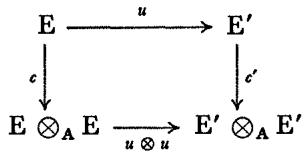
\includegraphics[keepaspectratio]{images/part004_6ed4336b.jpg}}

It is immediately verified that the identity mapping is a morphism, that the composition of two morphisms is a morphism and that every bijective morphism is an isomorphism.

Examples. (1) The canonical isomorphism \(\mathbf{A} \to \mathbf{A} \otimes_{\mathbf{A}} \mathbf{A}\) (II, § 3, no. 5) defines an A-cogebra structure on \(\mathbf{A}\) .

\begin{enumerate}
\def\labelenumi{(\arabic{enumi})}
\setcounter{enumi}{1}
\item
  Let E be a cogebra, c its coproduct and \(\sigma\) the canonical automorphism of the A-module \(E \otimes_{A} E\) such that \(\sigma(x \otimes y) = y \otimes x\) for \(x \in E\) , \(y \in E\) ; the A-linear mapping \(\sigma \circ c\) defines a new cogebra structure on E. With this structure E is called the opposite cogebra to the given cogebra E.
\item
  Let B be an A-algebra and let \(m:B \otimes_{A} B \to B\) be the A-linear mapping defining multiplication on B ( \(\S 1\) , no. 3). The transpose \(^{t}m\) is then an A-linear mapping of the dual \(B^{*}\) of the A-module B into the dual \((\mathbf{B} \otimes_{\mathbf{A}} \mathbf{B})^{*}\) of the A-module \(B \otimes_{A} B\) . If also B is a finitely generated projective A-module, the canonical mapping \(\mu:B^{*} \otimes_{A} B^{*} \to (\mathbf{B} \otimes_{\mathbf{A}} \mathbf{B})^{*}\) is an A-module isomorphism (II, \(\S 4\) , no. 4); the mapping \(c = \mu^{-1} \circ ^{t}m\) is then a coproduct defining a cogebra structure on the dual \(B^{*}\) of the A-module B.
\item
  Let X be a set, \(\mathbf{A}^{(\mathbf{X})}\) the A-module of formal linear combinations of elements of X with coefficients in A (II, §1, no. 11) and \((e_{x})_{x\in\mathbf{X}}\) the canonical basis of \(\mathbf{A}^{(\mathbf{X})}\) . An A-linear mapping \(c:A^{(\mathbf{X})}\to\mathbf{A}^{(\mathbf{X})}\otimes_{\mathbf{A}}\mathbf{A}^{(\mathbf{X})}\) is defined by the condition \(c(e_{x})=e_{x}\otimes e_{x}\) and a canonical cogebra structure is thus obtained on \(\mathbf{A}^{(\mathbf{X})}\) .
\item
  Let \(\mathbf{M}\) be an A-module and \(\mathsf{T}(\mathbf{M})\) the tensor algebra of \(\mathbf{M}\) ( \(\S 5\) , no. 1); by II, \(\S 3\) , no. 9 there exists one and only one A-linear mapping \(c\) of the A-module \(\mathsf{T}(\mathbf{M})\) into the A-module \(\mathsf{T}(\mathbf{M}) \otimes_{\mathbf{A}} \mathsf{T}(\mathbf{M})\) such that, for all \(n \geqslant 0\) ,
\end{enumerate}

\[
c (x _ {1} x _ {2} \dots x _ {n}) = \sum_ {0 \leqslant p \leqslant n} (x _ {1} x _ {2} \dots x _ {p}) \otimes (x _ {p + 1} \dots x _ {n})\tag{3}
\]

for all \(x_{i} \in \mathbf{M}\) ( \(x_{1}x_{2}\ldots x_{n}\) denotes the product in the algebra \(\mathsf{T}(\mathbf{M})\) ). Thus \(\mathsf{T}(\mathbf{M})\) is given a cogebra structure.

\begin{enumerate}
\def\labelenumi{(\arabic{enumi})}
\setcounter{enumi}{5}
\tightlist
\item
  Let M be an A-module and S(M) the symmetric algebra of M (§ 6, no. 1); the diagonal mapping \(\Delta: x \mapsto (x, x)\) of M into M × M is an A-linear mapping to which there therefore corresponds a homomorphism S(Δ) of the A-algebra S(M) into the A-algebra S(M × M) (§ 6, no. 2, Proposition 3). On the other hand, in § 6, no. 6 we defined a canonical graded algebra isomorphism \(h \colon \mathbb{S}(\mathbf{M} \times \mathbf{M}) \to \mathbb{S}(\mathbf{M}) \otimes_{\mathbf{A}} \mathbb{S}(\mathbf{M})\) ; by composition we therefore obtain an A-algebra homomorphism
\end{enumerate}

\[
c = h \circ \mathbf {S} (\Delta): \mathbf {S} (\mathbf {M}) \rightarrow \mathbf {S} (\mathbf {M}) \otimes_ {\mathbf {A}} \mathbf {S} (\mathbf {M}),
\]

thus defining on \(\mathbf{S}(\mathbf{M})\) a cogebra structure. For all \(x\in \mathbf{M}\) , by definition \(\mathbf{S}(\Delta)(x) = (x,x)\) and the definition of \(h\) given in § 6, no. 6 shows that

\[
h ((x, x)) = x \otimes 1 + 1 \otimes x.
\]

It follows that \(c\) is the unique algebra homomorphism such that, for all \(x \in \mathbf{M}\) ,

\[
c (x) = x \otimes 1 + 1 \otimes x.\tag{4}
\]

As \(c\) is an algebra homomorphism, it follows that, for every sequence \((x_{i})_{1\leqslant i\leqslant n}\) of \(n\) elements of \(\mathbf{M}\) ,

\[
\begin{array}{r l} c (x _ {1} x _ {2} \dots x _ {n}) & = \prod_ {i = 1} ^ {n} (x _ {i} \otimes 1 + 1 \otimes x _ {i}) \\ & = \sum (x _ {i _ {1}} \dots x _ {i _ {p}}) \otimes (x _ {j _ {1}} \dots x _ {j _ {n - p}}) \end{array}\tag{5}
\]

the summation on the right hand side of (5) being taken over all ordered pairs of strictly increasing sequences (in some cases empty)

\[
i _ {1} <   i _ {2} <   \dots <   i _ {p}, \quad j _ {1} <   j _ {2} <   \dots <   j _ {n - p}
\]

of elements of \([1, n]\) , whose sets of elements are complementary. The element \(c(x_1 x_2 \ldots x_n)\) is an element of total degree \(n\) in \(\mathbb{S}(\mathbf{M}) \otimes_{\mathbf{A}} \mathbb{S}(\mathbf{M})\) and its component of bidegree \((p, n - p)\) is

\[
\sum_ {\sigma} \left(x _ {\sigma (1)} \dots x _ {\sigma (p)}\right) \otimes \left(x _ {\sigma (p + 1)} \dots x _ {\sigma (n)}\right)\tag{6}
\]

where the summation is taken over all permutations \(\sigma\in\mathbb{S}_{n}\) which are increasing in each of the intervals \([1,p]\) and \([p+1,n]\) .

\begin{enumerate}
\def\labelenumi{(\arabic{enumi})}
\setcounter{enumi}{6}
\tightlist
\item
  Let \(\mathbf{M}\) be an A-module and proceed with the exterior algebra \(\bigwedge (\mathbf{M})\) as with \(\mathbb{S}(\mathbf{M})\) in Example 6; the diagonal mapping \(\Delta : \mathbf{M} \to \mathbf{M} \times \mathbf{M}\) this time defines a homomorphism \(\bigwedge (\Delta)\) of the A-algebra \(\bigwedge (\mathbf{M})\) into the A-algebra \(\bigwedge (\mathbf{M} \times \mathbf{M})\) (§ 7, no. 2, Proposition 2); on the other hand there is a canonical graded algebra isomorphism
\end{enumerate}

\[
h: \bigwedge (\mathbf {M} \times \mathbf {M}) \rightarrow \bigwedge (\mathbf {M}) ^ {\mathrm{g}} \otimes_ {\mathbf {A}} \bigwedge (\mathbf {M})
\]

(§ 7, no. 7, Proposition 10), whence by composition there is an algebra homomorphism \(c = h \circ \bigwedge(\Delta): \bigwedge(M) \to \bigwedge(M)^{\mathfrak{g}} \otimes_{A} \bigwedge(M)\) , which can be considered as an A-module homomorphism \(\bigwedge(M) \to \bigwedge(M) \otimes_{A} \bigwedge(M)\) and which therefore defines on \(\bigwedge(M)\) a cogebra structure. It can be proved as in Example 6 that \(c\) is the unique algebra homomorphism such that, for all \(x \in M\) ,

\[
c (x) = x \otimes 1 + 1 \otimes x,\tag{7}
\]

whence, for every sequence \((x_{i})_{1\leqslant i\leqslant n}\) of elements of \(\mathbf{M}\) ,

\[
c \left(x _ {1} \wedge x _ {2} \wedge \dots \wedge x _ {n}\right) = \left(x _ {1} \otimes 1 + 1 \otimes x _ {1}\right) \wedge \dots \wedge \left(x _ {n} \otimes 1 + 1 \otimes x _ {n}\right)
\]

where the product on the right hand side is taken in the algebra

\[
\Lambda (\mathbf {M}) ^ {\mathfrak {g}} \otimes_ {\mathbf {A}} \Lambda (\mathbf {M});
\]

to calculate this product, consider, for every ordered pair of strictly increasing sequences \(i_1 < i_2 < \cdots < i_p\) , \(j_1 < j_2 < \cdots < j_{n-p}\) of elements of \([1, n]\) , whose sets of elements are complementary, the product \(y_1y_2\ldots y_n\) , where \(y_{i_h} = x_{i_h} \otimes 1 (1 \leqslant h \leqslant p)\) and \(y_{j_k} = 1 \otimes x_{j_k} (1 \leqslant k \leqslant n - p)\) and the sum is taken over all these products. As the graded algebra \(\bigwedge (\mathbf{M})^{\mathfrak{g}} \otimes_{\mathbf{A}} \bigwedge (\mathbf{M})\) is anticommutative and the elements \(x_i \otimes 1\) and \(1 \otimes x_i\) are of total degree 1, by §4, no. 6, Lemma 3 and Lemma 1,

\[
\begin{array}{r l} c (x _ {1} \wedge x _ {2} \wedge \dots \wedge x _ {n}) & = \sum (- 1) ^ {\nu} (x _ {i _ {1}} \wedge \dots \wedge x _ {i _ {p}}) \otimes (x _ {j _ {1}} \wedge \dots \wedge x _ {j _ {n - p}}) \end{array} \tag {8}
\]

v being the number of ordered pairs \((h, k)\) such that \(j_{k} < i_{h}\) and the summation being taken over the same set as in (5). The element \(c(x_{1} \wedge \cdots \wedge x_{n})\) is of total degree n in \(\bigwedge(\mathbf{M})^{\mathbf{g}} \otimes_{\mathbf{A}} \bigwedge(\mathbf{M})\) and its homogeneous component of bi-degree \((p, n - p)\) is equal to

\[
\sum_ {\sigma} \varepsilon_ {\sigma} (x _ {\sigma (1)} \wedge \dots \wedge x _ {\sigma (p)}) \otimes (x _ {\sigma (p + 1)} \wedge \dots \wedge x _ {\sigma (n)})\tag{9}
\]

the summation being taken over permutations \(\sigma\in\mathfrak{S}_{n}\) which are increasing in each of the intervals \([1,p]\) and \([p+1,n]\) .

When in future we speak of \(\mathbf{A}^{(\mathbf{X})}\) , \(\mathsf{T}(\mathbf{M})\) , \(\mathsf{S}(\mathbf{M})\) or \(\bigwedge (\mathbf{M})\) as cogebras, we shall mean, unless otherwise mentioned, with the cogebra structures defined in Examples 4, 5, 6 and 7 respectively.

\begin{enumerate}
\def\labelenumi{(\arabic{enumi})}
\setcounter{enumi}{7}
\tightlist
\item
  Let E, F be two A-cogebras and c, \(c'\) their respective coproducts. Let \(\tau:(\mathbf{E} \otimes_{\mathbf{A}} \mathbf{E}) \otimes_{\mathbf{A}} (\mathbf{F} \otimes_{\mathbf{A}} \mathbf{F}) \to (\mathbf{E} \otimes_{\mathbf{A}} \mathbf{F}) \otimes_{\mathbf{A}} (\mathbf{E} \otimes_{\mathbf{A}} \mathbf{F})\) denote the associativity isomorphism such that \(\tau((x \otimes x') \otimes (y \otimes y')) = (x \otimes y) \otimes (x' \otimes y')\) for \(x, x'\) in E and \(y, y'\) in F. Then the composite linear mapping
\end{enumerate}

\[
\mathrm{E} \otimes_ {\mathrm{A}} \mathrm{F} \xrightarrow {c \otimes c ^ {\prime}} (\mathrm{E} \otimes_ {\mathrm{A}} \mathrm{E}) \otimes_ {\mathrm{A}} (\mathrm{F} \otimes_ {\mathrm{A}} \mathrm{F}) \xrightarrow {\tau} (\mathrm{E} \otimes_ {\mathrm{A}} \mathrm{F}) \otimes_ {\mathrm{A}} (\mathrm{E} \otimes_ {\mathrm{A}} \mathrm{F})
\]

defines a cogebra structure on the A-module E \(\otimes_{\mathbf{A}}\mathbf{F}\) , called the tensor product of the cogebras E and F.

Let E be a cogebra and \(\Delta\) a commutative monoid. A graduation \((\mathrm{E}_{\lambda})_{\lambda\in\Delta}\) on the A-module E is said to be compatible with the coproduct c of E if c is a graded homomorphism of degree 0 of the graded A-module E into the graded A-module (of type \(\Delta\) ) \(E\otimes_{A}E\) , in other words (II, §11, no. 5) if

\[
\mathrm{c} (\mathrm{E} _ {\lambda}) \subset \sum_ {\mu + \nu = \lambda} \mathrm{E} _ {\mu} \otimes_ {\mathbf {A}} \mathrm{E} _ {\nu}.\tag{10}
\]

In what follows, we shall most often limit our attention to graduations of type N compatible with the coproduct; a cogebra with such a graduation will also be called a graded cogebra. If F is another graded cogebra, a graded cogebra morphism \(\phi:E\to F\) is by definition a cogebra morphism (Definition 2) which is also a graded homomorphism of degree 0 of graded A-modules.

Examples. (9) It is immediate that the cogebras \(\mathsf{T}(\mathbf{M})\) , \(\mathsf{S}(\mathbf{M})\) and \(\bigwedge (\mathbf{M})\) defined above are graded cogebras.

